\documentclass[../../main.tex]{subfiles}
\begin{document}

This section will provide a description of the elements of the given pan-tilt system as well as an analysis of possible approaches to satisfy the problem description described in section \ref{sec:ProblemDescription}.

\subsection{Description of Physical Setup}
The pan-tilt system is made of aluminium extrusions and can be divided into two sections, a stationary lower section and a upper movable section. The movable section consists of two \textit{frames}, the pan frame and the tilt frame. The tilt frame is a simple square, and the pan frame is u-shaped with the tilt frame attached inside as illustrated on figure \ref{fig:Pan_Tilt_Drawing}. The tilt frame can rotate freely while the pan frame is limited in its rotation to around $\SI{160}{\degree}$ by mechanical limitation.

From initial experiments with the pan-tilt system it is found that significant friction is present in joints and bearings. It is also found that the friction varies according to the position of the frame. Probably these irregularities stem from the physical setup being poorly constructed, as it is visibly skewed.  

Each frame is actuated by a \SI{12}{\volt} DC motor equipped with an incremental encoder \cite{}. The resolution of the encoders is 360 counts per revolution of the output shaft. The encoders make it possible to determine an offset from the initial position. The gearing between the motors and the frames on the robot is 3:1, so the frame experiences one revolution for every three revolutions the motor experiences. Hall effect sensors \cite{} provide an index signal for each frame. The index signals are used to provide a reference point for the incremental encoders. From the change in position relative to the time, the velocity of the motor can be calculated. Both motors are connected to an H-bridge, which can be enabled with a PWM-signal to control the voltage over the motors. In accordance with the datasheet of the H-Bridge, L6203 \cite{} \ref{sec:digital_appendix}, it requires a PWM frequency typically around \SI{30}{\kilo\hertz} and up to \SI{100}{\kilo\hertz} to function. The H-bridge also makes is possible to change the polarity of the voltage supplied, yielding a change in the motors turning direction.

\subsection{Controller Design}

Figure \ref{fig:Open_Close_loop} shows a simple \textit{controller} setup.
The plant is the system which is to be controlled. The controller outputs a control signal which is the input to the plant. 
In this project the plant would be an electric motor for which the control signal could be a voltage and the output could be an angular velocity.
If a perfect model of the plant exists, and no external disturbances act on the system, a controller can be designed that controls the plant purely based on a reference input. This type of system would be classified as open-loop. In reality, such a system cannot be obtained, so to properly control the system, it is beneficial to monitor the output of the plant. The output is subtracted from the reference, yielding an error used as input for the controller. This type of feedback yields a closed loop system and makes the system more robust. 

The problem description states that a position controller has to be designed, however such a controller can take on many forms, leading to different design approaches and methods. Generally speaking, controller design can be divided into two categories, classical control, which operates in the frequency domain, and modern control which operates in the time domain. Both approaches will be examined in this section.





% Instead of utilising the integral term to correct the steady state error, a feedforward loop can be introduced. Feedforward eliminates the steady state error by adding the error between the output and the reference at steady state. This however requires knowledge about the system at steady state, and can therefore not be applied if information about the system in steady state is not available. 




% When the control signal goes beyond the saturation limits will keep winding up yielding a bigger difference between the wanted control signal and the saturated control signal. This means the control signal will take longer to return to the unsaturated area. To counteract this behaviour anti-windup can be added to the controller. Multiple methods for implementing anti-windup exists, only the methods back-calculation and conditional integral will be examined. Conditional integral is the simplest method, where the integral term is only evaluated when the control signals not is in beyond the saturation limits. The principle behind the back-calculation method is to subtracting the unsaturated signal from the saturated, and the adding a fraction of the difference to the integral input.  

% can be taken into account by implementing saturation in the modelling of controller and plant.
%Different approaches to anti-windup is available and is often related to the controller in question.

% When controlling the pan-tilt system a user-input is required with a position for the motors. When 
% As a voltage is applied across a motor, a current will run through the coils of the motor, while the motor will start spinning with an angular velocity. Current and velocity are two aspects of the motors that change at a higher rate than the position of the motor, while also influencing the position of the motor. 

% Using a single \textit{controller} it is not a problem as long as the relation between the current and position remains the same. 
% However if any noise is introduced to the system altering the relation between the current and position, the response of the position controller is retarded. This is due to the current changing rapidly compared to the position. 

%Adding a controller dealing with the velocity and current and implementing the controllers in cascade, the outer controller is isolated from the faster changes of velocity and current, leaving the designated controllers to control them. When implementing the controllers in cascades, the position controller feeds the velocity controller with the velocity reference point and the velocity controller feeds the current controller, which results in the required current for the motor to achieve the desired position. This means that the velocity and current controller will deal with any noise such as friction, thus achieving a faster compensation to noise and a faster response overall. However this introduces three controllers, which have to be tuned individually, making the intuitive process of tuning more challenging \cite{CascadeControl}.
%Anti windup

\begin{figure}[H]
    \centering
    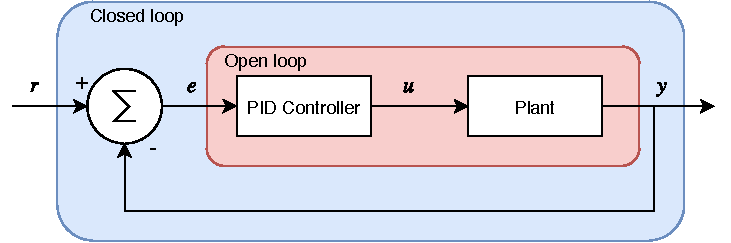
\includegraphics[width=0.7\textwidth]{Sections/Miscellaneous/Images/Open_closed_Diagram.pdf}
    \caption{Figure illustrating the concept of controller setup highlighting the open- and closed-loop concepts. }
    \label{fig:Open_Close_loop}
\end{figure}





\subsection*{Classical Control Methods}\label{subsec:classic_control}


A traditional method for designing a controller for a motor is to use a PID-controller. Though many controller configurations using parts of the PID-controllers design exists, only the full PID-controller will be examined. The block diagram of a PID-controller can be seen on figure \ref{fig:anti-windup}. As seen on the block diagram
a PID-controller utilises a feedback loop. The controller consist of three terms: a proportional term, an integral term and a derivative term. Each term is evaluated separately and then combined to yield the output of the controller. If only the proportional term is used, a steady state error between the output and the reference will always be present. Therefore the integral term is introduced to eliminate the steady state error, as the integral will keep increasing until there is no steady state error. The derivative term adds anticipatory action based on the trend of the error. \cite{}




%I tilfælde med dette system 
% \begin{equation}\label{eq:feedforward}
%     u_{ff}=\frac{1}{G(0)}r(t)
% \end{equation}
% \begin{figure}[]
%     \centering
%     \includegraphics[width=0.7\textwidth]{Sections/Miscellaneous/Images/PID-control-diagram.png}
%     \caption{Block diagram of a PID-controller with an additional feedforward implemented.}
%     \label{fig:PID_controller}
% \end{figure}

% The proportional term is proportional to the error, but leaving the output with a steady state error, due to the term always requiring an error to function. To correct this steady state error, feedforward can be introduced, where the proportional signal is added as seen on equation \ref{eq:feedforward}, where $G$ is the transfer function of plant and $r$ is the setpoint.
% \begin{equation}\label{eq:feedforward}
%     u_{ff}=\frac{1}{G(0)}r(t)
% \end{equation}
% However feedforward is sensitive to modelling uncertainties, due to it heavily relying on the design of the plant. Instead the integral term can be implemented, integrating the error thus eliminating the steady state error. To increase the settling time of the controller the derivative term can be added, which is an anticipatory term looking at the trend of the error, thus making it possible to change the direction of the signal, if overshoot or oscillating tendencies occurs. However the derivative term is vastly sensitive to noise, making it necessary to filter the signal upon implementation of the controller. 

To achieve a desired response of the system, the different gains of the PID-controller must be found. Finding gains for the PID-controller different methods are available each with different advantages. A method is \textit{pole placement}, where the location of poles in the closed-loop system are strategically placed. This introduces the prerequisite, that an accurate model of the system must be known. Furthermore the designer must know, where to place the poles to achieve the desired response.
The root locus provides a method of analysing movement of the poles as an increasing gain is applied to the system. The method makes it possible to tweak the gain until the desired response is achieved.
If no model of the plant is available other means for tuning is present. Two heuristic methods known as Ziegler-Nichols methods exist. One is based on creating a marginally stable system, and the other is based on the open-loop step response of the plant. Only the latter will be examined further. This method, assumes that the plant can be described by a first order delayed system. 


% Having a transfer function of a given plant, $G(s,K)$, with an unknown parameter K, it is possible to describe the movement of the poles in the s-plane using the root locus method. By looking at the rise time, overshoot and settling time it is possible to estimate where in the s-plane the poles can be placed to ensure the desired behavior of the system. %Limitations for the placement of the poles can be found. 
% With the root locus method, it is possible to tweak the controller in such a manner, that the system satisfies the requirements.

Physical systems have limitation such as maximum ratings. When modelling such systems these limitations can be taken into account by introducing saturation to the control signal. The saturation will level the signal at the saturation limit if the signal exceeds the saturation limits. Having a system in saturation the integral term will continue to windup as long as an error is present between the reference and the output. This is not a desired behaviour, since it will take time for the integral term to decrease for the control signal to go below the saturation limit. To circumvent this, anti-windup can be implemented. %However this is not a desired behaviour, creating a slower response of the control signal, $v$, goes below saturation. Figure \ref{fig:anti-windup} illustrates the implementation of back calculation for a PID-controller. When the system is in saturation, and therefor not able to increase, the control signal $u$ is constant. The time tracking constant, $\frac{1}{T_t}$ determines how quick the integrator is changed.
When implementing anti-windup it can be executed using back-calculation or conditional integration. The implementation of back calculation can be seen on figure \ref{fig:anti-windup}. This approach feeds a fraction of the difference between the commanded output signal and the saturated signal back to the integrator. This way keeping the commanded output signal close to the saturation limits, while in saturation. Conditional integration works by feeding zero into the integrator, thus keeping the integration term constant, when the control signal is saturated. 

\begin{figure}
    \centering
    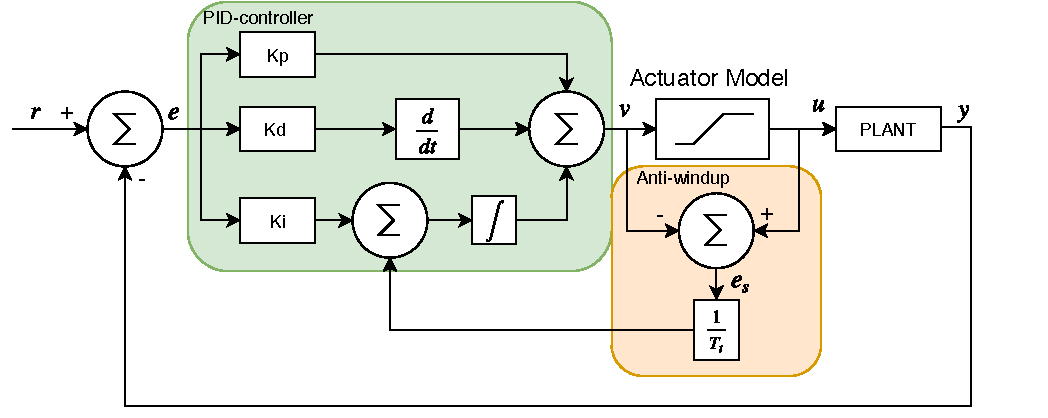
\includegraphics[width=0.7\textwidth]{Sections/Miscellaneous/Images/PID-Anti-windup-BackCalc.pdf}
    \caption{Block diagram of a PID-controller including anti-windup implemented using back calculation. $T_t$ is the tracking time constant and $e_s$ is the saturation error.}
    \label{fig:anti-windup}
\end{figure}

Instead of using a single controller for the plant, sometimes it can be beneficial to implement multiple controllers in a cascaded design as shown on figure \ref{fig:cascaded_design_analysis}. Here, the plant is perceived as multiple simpler plants that feed into each other. The outermost control loop will then supply the reference signal for the next and so on. If designed correctly, this design will provide better noise rejection and lower sensitivity to parameter variations. This is because disturbances acting on the inner loop will be isolated from, and ideally invisible to the outer control loops. On the pan-tilt system a cascade constituting three controllers would be a inner current controller, a velocity controller and then an outer position controller.

\subsubsection*{Modern Control Methods}
%explain states -> state space form
A system can be described based on the dynamics of the states found in the system. For the DC motor example, the states could be current, angular velocity and angular position. The dynamics can be presented using the state space form shown in equation \ref{eq:gen_statespace}.

\begin{equation}\label{eq:gen_statespace}
    \begin{split}
        \Dot{x}&=Ax+Bu \\
        y&=Cx \qquad ,%\\
        %u&=Fx
    \end{split}
\end{equation}

where $A$ is the system matrix, $B$ is the input matrix, $C$ is the output matrix,  $x$ is a vector containing the states and $u$ is a vector containing external control signals.
Modern control aims to control the states in the system via state feedback, which introduces the control law seen in equation \ref{eq:state_feedback}.

\begin{equation}\label{eq:state_feedback}
    u = F x \qquad ,
\end{equation}

where $F$ is the feedback matrix, which can be designed to yield the desired system response.


% Modern control methods utilises state feedback represented as a block diagram on figure \ref{fig:Integral_Diagram}. A simple state space feedback can be described as seen in equation \ref{eq:gen_statespace}, where $A$ is the system matrix, $B$ is the input matrix, $x$ is the state, $u$ is the control signal, $y$ is the output, $C$ is the  and $F$ is the state feedback matrix. 



One approach to design the feedback matrix is pole assignment, where the feedback matrix is calculated to yield specific closed loop poles in order to achieve a desired response. This requires the designer to decide exactly where the poles should be placed, which for somewhat complex systems can be difficult.
A Different approach is using the linear quadratic regulator method. This algorithm is based around the minimising of a cost function concerning the optimisation of operating a linear system. This method provides a way to apply a weight to each state and each control signal and thereby influence which will be prioritised higher. As an example, the states can be prioritised highly giving a fast response, at the cost of more aggressive control signals.

Since both of the these design methods are based on a linear model of the system, it is a prerequisite that a very accurate model of the plant, which is defined by the $A$ and $B$ matrices, is known. 

\begin{figure}
    \centering
    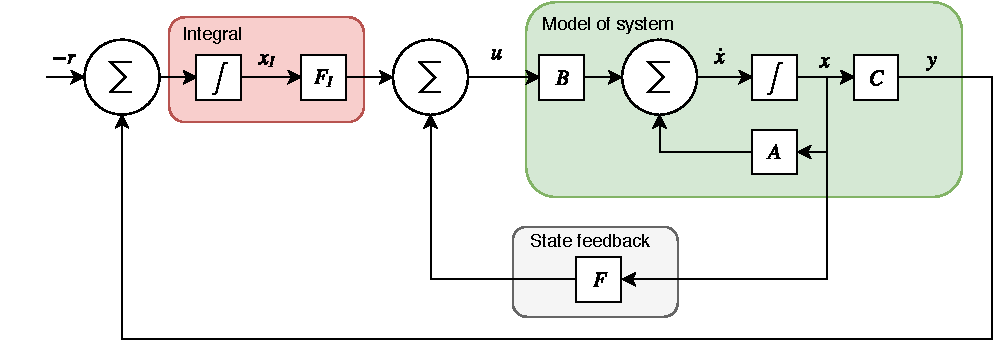
\includegraphics[width=0.7\textwidth]{Sections/Miscellaneous/Images/Statefeedback_Integral.pdf}
    \caption{Block diagram of an integral controller.}
    \label{fig:Integral_Diagram}
\end{figure}

A way to reduce some of the issues from uncertainties about the plant, is to include integral action as seen on figure \ref{fig:Integral_Diagram}. The integral feedback provides zero steady state error by integrating the error. Taking basis in the state space form equation \ref{eq:gen_statespace} and adding an additional feedback, the input is given as described in equation \ref{eq:input_integral}.  

\begin{equation}\label{eq:input_integral}
        u=Fx+F_Ix_I \qquad , 
\end{equation}

where $F$ is the state feedback matrix, $F_I$ is the integral matrix and $X_{I}$ is described in equation \ref{eq:integral_xi}.

\begin{equation}\label{eq:integral_xi}
    x_I(t)=\int_0^t y(\tau)-r(\tau)\,d\tau \qquad ,
\end{equation}

where $t$ is the time, $y$ is the output, $r$ is the reference and $\tau$ is the integration variable.

\begin{figure}
    \centering
    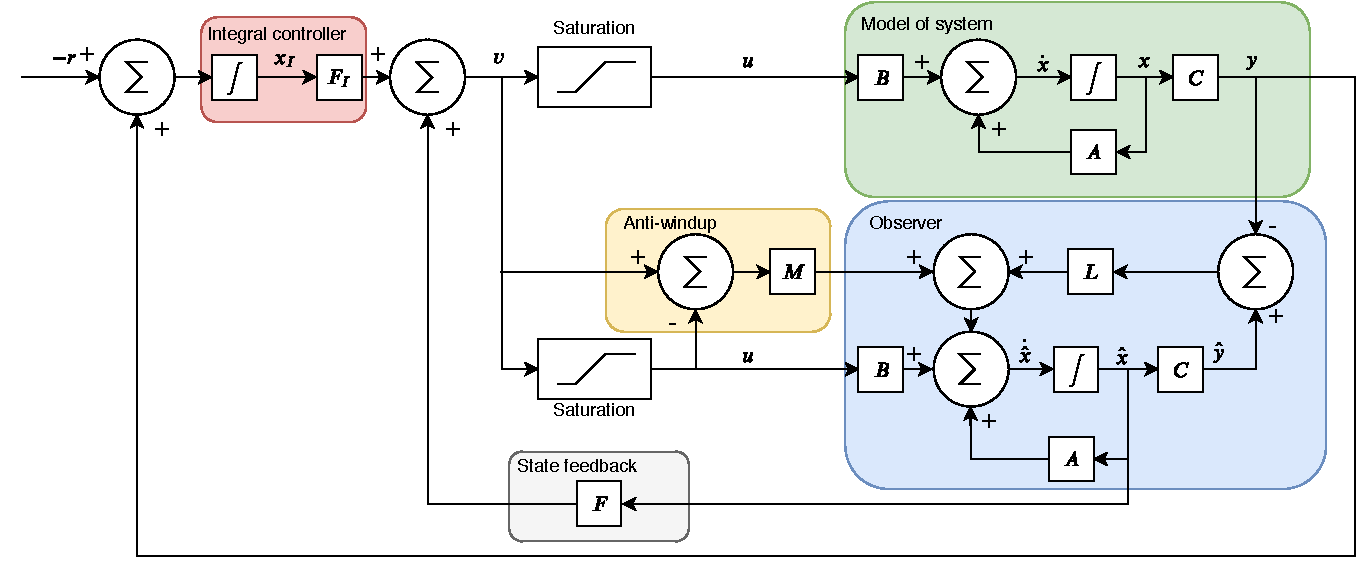
\includegraphics[width=0.9\textwidth]{Sections/Miscellaneous/Images/Anti_Windup_Integral_Observer.pdf}
    \caption{Block diagram of an integral controller with observer and anti-windup.}
    \label{fig:Integral_Observer_Diagram}
\end{figure}

State feedback requires that every state is measured, which is rarely possible. However means to estimate states of a given system are available. The estimation can be achieved by introducing an observer to the system, which is illustrated on figure \ref{fig:Integral_Observer_Diagram}. The observer aims to mirror the plant and by that making it possible to approximate a given state.
The observer introduces an observer gain, $L$, which is proportional with the difference between the output from the plant and the estimated observer output. The observer state space model is as seen in equation \ref{eq:Obs_state_space}, where $\hat{x}$ is the estimated state and $\hat{y}$ is the estimated output.
\begin{equation}\label{eq:Obs_state_space}
    \begin{split}
        \Dot{\hat{x}}&=A\hat{x}+Bu+L(C\hat{x}-y)\\
        \hat{y}&=C\hat{x}
    \end{split}
\end{equation}

As with the classical control, saturation might be considered in modern control. This can be handled by introducing a matrix $M$, as seen in figure \ref{fig:Integral_Observer_Diagram}, which can alter the system dynamics when in saturation.

% To take into account that there are physical limitation in form of saturation an anti-windup in form of the gain $M$ on figure \ref{fig:Integral_Observer_Diagram} can be added. The anti-windup subtracts $v$ with the control signal, $u$ and multiplies it with the gain, $M$. If there is a different it prevent the integral term to windup. 
% If saturation occur the dynamic of the observer controller changes to:
% \begin{equation}\label{eq:anti-windup_state_space}
%     \begin{split}
%         \Dot{\hat{x}}&=A\hat{x}+LC\hat{x}+MF\hat{x}\\
%         \hat{y}&=C\hat{x}
%     \end{split}
% \end{equation}

% Thus the equivalent state space model of an integral controller with an observer and anti-windup is as seen on equation \ref{eq:state_space_modern_control}.

% \begin{equation}\label{eq:state_space_modern_control}
% \begin{split}
% \begin{bmatrix}
%         \dot{x} \\
%         \dot{\hat{x}}\\
%         \dot{x}_I
%     \end{bmatrix} &=
%     \begin{bmatrix}
%         A & BF & BF_I \\
%         -LC & A+BF+LC & BF_I \\
%         C & 0 & 0
%     \end{bmatrix}
%     \begin{bmatrix}
%         x \\
%         \hat{x} \\
%         x_I
%     \end{bmatrix}
%     + 
%     \begin{bmatrix}
%     0\\
%     0\\
%     -I
%     \end{bmatrix}
%     r \\
%     y &= \begin{bmatrix}
%         C & 0 & 0
%     \end{bmatrix}     
%     \begin{bmatrix}
%         x \\
%         \hat{x} \\
%         x_I
%     \end{bmatrix}, 
%     \end{split}
% \end{equation}
% where $r$ is the reference and $\Dot{\hat{x}}$ is described by equation \ref{eq:anti-windup_state_space} when saturation occurs.

\subsection*{Implementation}
%modelling, continuous vs discrete
%more implementing methods
Upon designing a controller it is important to keep in mind that an actual implementation is discrete rather than continuous when implemented in software. The plant for which the controller is designed is continuous making it difficult to match the requirements of the discrete controller. The controller can be designed continuous and then discretizised to render the possibility of implementation. Another approach is discretizising the plant and then designing the controller discrete. However this requires a method of mapping from the domains. Different means of mapping from the continuous domain (s-domain) to the discrete domain (z-domain) is available such as the trapezoidial rule, forward rectangular rule and the backward rectangular rule. 
\begin{figure}
    \centering
    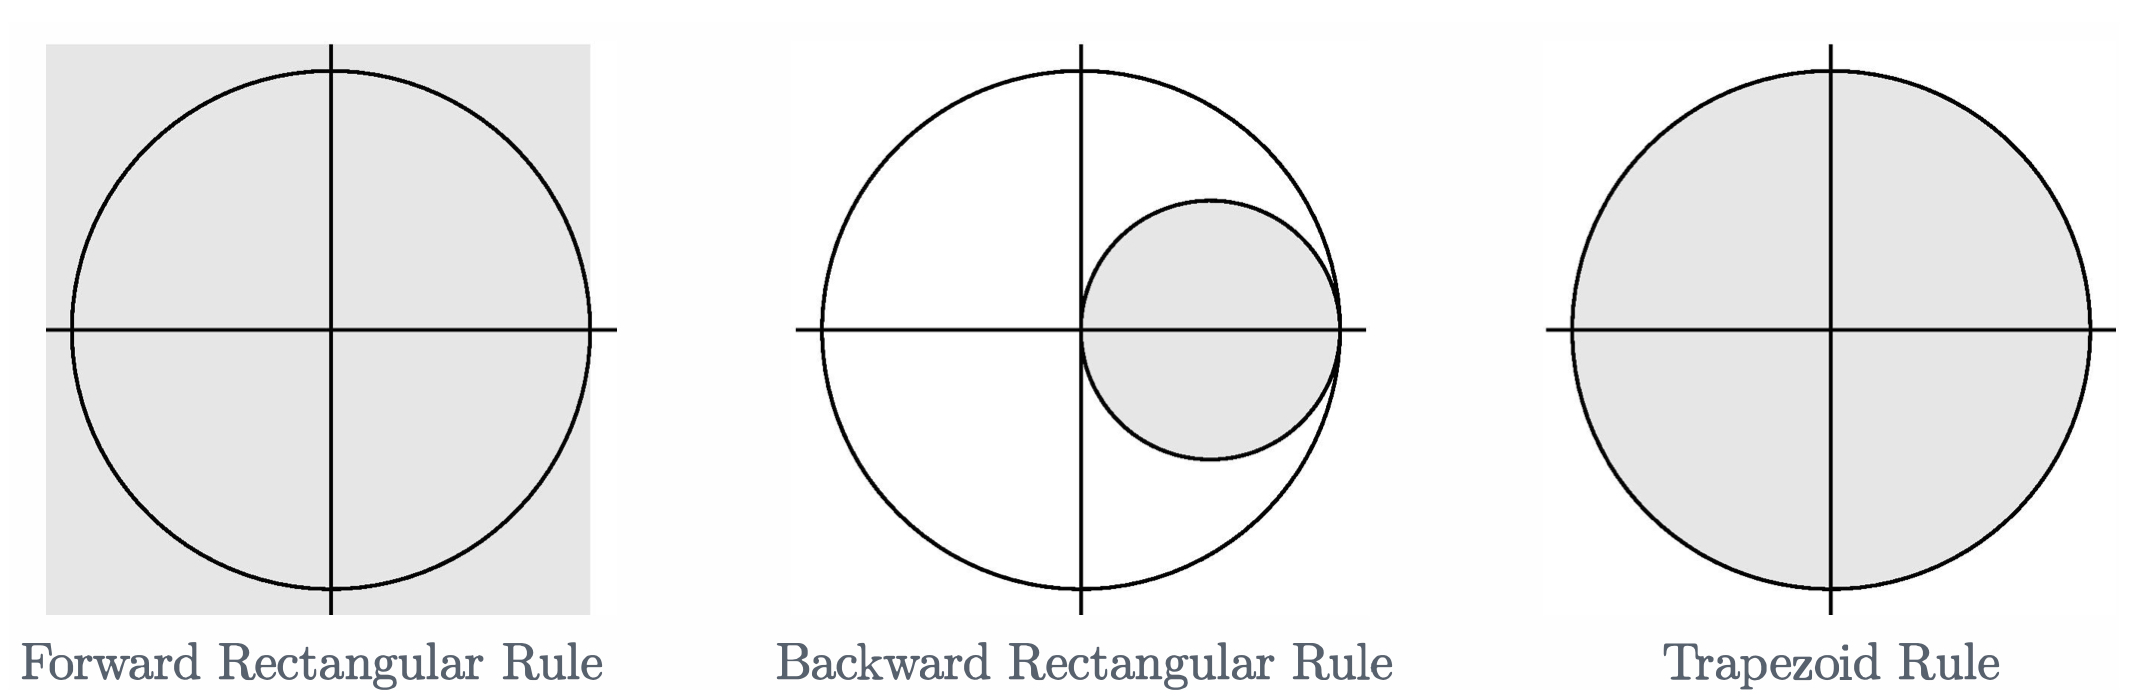
\includegraphics[width = 0.7\textwidth]{Sections/Miscellaneous/Images/Trapezoid_rule.jpeg}
    \caption{Illustration of mapping from the continuous s-domain to the discrete z-domain using different approaches.}
    \label{fig:mapping_s_to_z}
\end{figure}
Using the forward rectangular rule to map from the s to the z-domain, the entire left-half plane of the s-domain is mapped into the z-domain into a rectangular shape. The forward rectangular rule maps the left-half plane of the s-domain into a circle placed in the right-half of the z-domain. The trapezoidial rule fits the left-half plane of the s-domain into the unit-circle of the z-domain. The phenomenons are illustrated on figure \ref{fig:mapping_s_to_z}.  

Implementing the discrete controller can be done as seen in equation \ref{eq:discrete_control}, utilising the Tustins method. Tustins method is based on the trapezoidial rule, and dictates a certain way of implementing the integral and thereby the differential part.
\begin{equation}\label{eq:discrete_control}
\begin{split}
        u(kT+T)=&k_Pe(kT+T)+u_1(kT)\\ &+ k_I\frac{T}{2} \cdot (e(kT+T)+e(kT))\\ &+k_D \frac{2}{T}(e(kT+T)-e(kT))-u_D(kT) \quad ,
\end{split}
\end{equation}

where $u(s)$ is the control signal in continuous time and $u(kT+T)$ is the control signal in discrete time. $T$ is the sampling time, $e$ is the error and $k_p$, $k_I$ and $k_D$ are the PID gains.

As seen from equation \ref{eq:discrete_control} the terms depend on the sampling time, thus it needs to be known. A rule of thump state that the sampling frequency for a discrete controller, should be approximately 20 times larger than the closed-loop bandwidth of the system \cite{Design_Of_Digital_Control_Systems_NOTE}. 

%  In time-domain each term can be described as in equation \ref{eq:time-domain-PID-controller}.
% \begin{equation}
%     \label{eq:time-domain-PID-controller}
%     u(t) = u_P(t) + u_I(t) + u_D(t)
% \end{equation}
% To discretize, each term will be evaluated at time $kT+T$, with $k$ being sample number.
% \begin{equation}
%     u(kT+T) = u_P(kT+T) + u_I(kT+T) + u_D(kT+T)
% \end{equation}
% By multiplying the error $e$ with gain $k_P$, the proportional term is:
% \begin{equation}
%     u_P(kT+T) = k_P e (kT+T)
%     \label{eq:P-Term_discretized}
% \end{equation}
% To get the integral term a numerical integration of the error is necessary. To get the average error between the error at time $kT$ and $kT+T$ the trapezoidal method is used for integration, shown in equation \ref{eq:TrapezoidalIntegrationMethod}:
% \begin{equation}
% \label{eq:TrapezoidalIntegrationMethod}
%     \int_{kT}^{kT+T}e(\tau) d\tau \approx T\left(\frac{e(kT+T) + e(kT)}{2} \right)
% \end{equation}
% To make sure the integral term keeps increasing while an error is present in the system, the integral at previous sample $kT$ is added. Now the integral term is as follows:
% \begin{equation}
%     u_I(kT+T) \approx u_I(kT) + k_I\frac{T}{2}(e(kT+T) + e(kT))
%     \label{eq:I-term-Discretized}
% \end{equation}
% The derivative term is obtained by integrating equation \ref{eq:startDerivativeTerm}, to obtain equation \ref{eq:DerivativeTermPartiallyIntegrated}:
% \begin{equation}
%     \label{eq:startDerivativeTerm}
%     u_D(t)=k_D\dot{e}(t)
% \end{equation}
% \begin{equation}
% \label{eq:DerivativeTermPartiallyIntegrated}
%     k_De(kT+T) = \int_{0}^{kT}u_D(\tau)d\tau + \int_{kT}^{kT+T}u_D(\tau)d\tau
% \end{equation}
% Which then can be written as:
% \begin{equation}
%     u_D(kT+T) \approx k_D\frac{2}{T}(e(kT+T)-e(kT)) -u_D(kT)
%     \label{eq:D-Term_discretized}
% \end{equation}
% From equation \ref{eq:P-Term_discretized}, \ref{eq:I-term-Discretized} and \ref{eq:D-Term_discretized} the control output of the discrete system is:
% \begin{equation}
%     u(kT+T) = k_P e (kT+T) + u_I(kT) + k_I\frac{T}{2}(e(kT+T) + e(kT)) + k_D\frac{2}{T}(e(kT+T)-e(kT)) -u_D(kT)
%     \label{eq:DisretizedModel}
% \end{equation}

\subsection*{Microcontroller}
Implementing at least two controllers on the same microcontroller and having to accommodate other tasks such as SPI and UART in parallel. It would be advantageous to implement some sort of scheduling algorithm. The easiest way of implementing a scheduling algorithm is by the use of an operating system (OS). Various types of operating systems exist, though in this project only two operating systems has been evaluated, Run To Complete Scheduler (RTCS) and FreeRTOS. The RTCS uses a cooperative scheduling algorithm, where the task voluntarily has to yield processing time on the CPU. This method provides a light weight overhead, though the risk of a task blocking the CPU is greater as no master can reallocate resources while another task i running. 
 % The run to complete scheduler (RTCS) constitutes such an algorithm and is based on a cooperative scheduling where a running task wont be interrupted by other tasks, unless the task voluntarily yield control. Thus to achieve a seemingly multitasking system all tasks must cooperate to prevent starvation of tasks. 
The FreeRTOS as standard uses a preemptive scheduling algorithm where a central master is responsible for the allocation of resources. The central master can preempt a task whenever it is wanted, therefore minimising the probability of starvation occurring. FreeRTOS does however provide a greater overhead compared to the RTCS. If time-critical tasks exists in the system, it is preferred to use a OS providing real-time capabilities. A real-time system ensures that important tasks is guaranteed to complete within a given time frame from when the task is signaled to run. FreeRTOS provides functionalities to operate as a real-time system, such as prioritisation of tasks.   

% could also be implemented, which opposed to the RTCS allow the scheduler to preempt tasks when the allocated CPU time of the task is used. Switching between tasks does however introduce overhead.\\

% Ideally controllers implemented on the microcontroller would need and use new data as soon as it is sampled. Intertask communication also demands management of datasharing, since it is usually unsafe for two tasks to access the same specific data. To have the system use a scheduling algorithm and ensure reliable performance, an operating system (OS) can be used. The real-time operating system (RTOS) is an OS using preemptive scheduling and is intended to have tasks process data as it comes in. It also allows for prioritization of tasks, so timing of more time-critical tasks does not become compromised. 



%Another algorithm is FreeRTOS, which schedules tasks based on priority and CPU time and constitutes a real time operating system (RTOS). In addition FreeRTOS also provide a broad range of predefined functionality regarding queues and semaphores.  


\end{document}